\chapter{Design}

The design of Snapstore had two steps. The first was to identify the purposes of a version control system. The six purposes of a version control system identified in \cite{RossoJackson} were used.

The next step was to create a conceptual model composed of concepts that fulfilled the purposes of a version control system. These concepts were invented in a way that is aligned with conceptual design theory \cite{Jackson}. That is, they were each had a motivating purposes, they were not redundant or overloaded, and they were uniform. A mapping of each Snapstore concept to its motivating purpose is shown in Table 3.1. The $\mapsto$ symbol stands for ``is a subpurpose of''. A graphical representation of the conceptual model, using the notation for extended entity-relationship as used in \cite{Jackson}, is shown in Figure 3-1.

\vspace{6mm}

\begin{table}
\begin{tabular}{ |p{6cm}||p{9cm}|  }
 \hline
 \textbf{Concept} & \textbf{Motivating Purpose} \\[8pt]
 \hline
 Snapshot & Making a set of changes to a file persistent\\[8pt]
 Create, Update, Rename, and Delete Snapshot & Track various types of changes to a file $\mapsto$ making a set of changes to a file persistent\\[8pt]
 Snapstore Folder & Create, read, and update files $\mapsto$ making a set of changes to a file persistent\\[8pt]
 Tracked File & Mark files whose changes should be saved $\mapsto$ making a set of changes to a file persistent\\[8pt]
 Untracked File & Mark files whose changes should be ignored $\mapsto$ making a set of changes to a file persistent\\[8pt]
 \hline
 Group & Grouping logically related changes together\\[8pt]
 Tag & Represent and record coherent points in history\\[8pt]
 \hline
 Upstream Repository & Synchronize changes of collaborators\\[8pt]
 Branch & Support parallel lines of work\\[8pt]
 Local Repository & Do work in disconnected mode\\[8pt]
 \hline
\end{tabular}
\caption{VCS purpose to concept mapping for Snapstore}
\end{table}

\begin{figure}
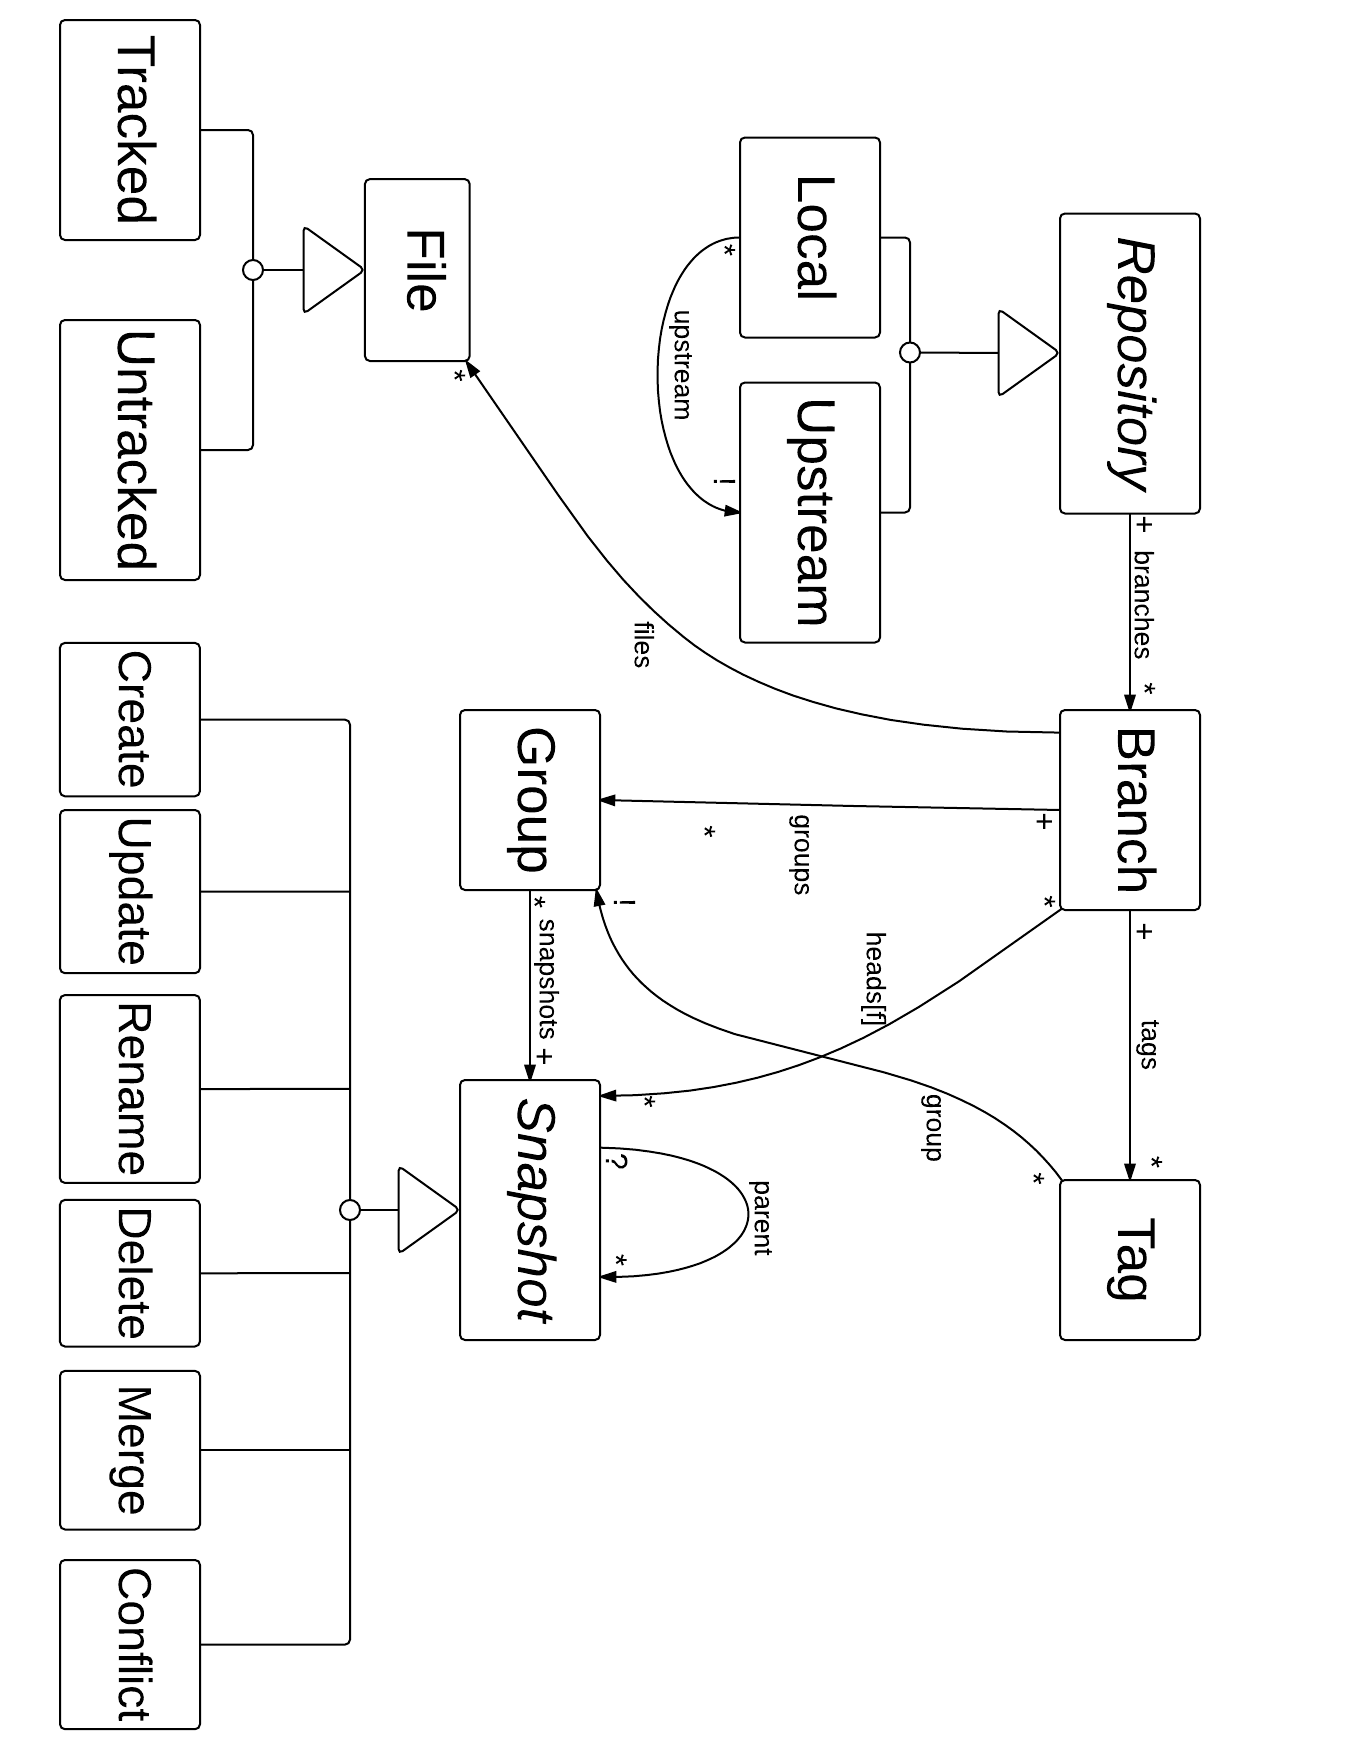
\includegraphics[max width= \linewidth]{ConceptModel}
\caption{Concept Model of Snapstore.}
\label{arm:fig1}
\end{figure}

\section{Data Storage - Snapshot}

Persistent data storage in Snapstore is achieved with the notion of a \textit{snapshot}. The snapshot is a saved state of a file. Snapshots record updates, renames, moves, deletes, and merges. Records of the many operations enable all VCS features of Snapstore. The \textit{head} snapshot for any given file is the most recent snapshot made for that file and the current content of that file. 

A snapshot is either a create, an update, a rename, or a delete snapshot. This distinction dictates the values of the snapshot fields. Create snapshots have no parent. Update snapshots have a parent, a child, and content. Rename snapshots have a different filename than their parent. Delete snapshots have no content.

All snapshots have parent snapshots and child snapshots. The snapshots of a file are related by the graph they create with these parent/child relationships. This ordering forms the snapshot graph described in the tutorial section. The snapshot graph is guaranteed to be an in-order description of snapshots a specific client has made to a file in a branch. Each unique (branch, file) tuple is represented by its own snapshot graph. A snapshot can have multiple parents if it is the result of a merge operation.

Any file, identified by its snapshot graph, can either be tracked or untracked. Untracked files will not create snapshots and will not affect the local or upstream repositories.

\section{Grouping Changes - Group}

A \textit{group} is an assembly of related snapshots. A group must contain at least one snapshot, but there are no restrictions on what kinds of snapshots can be in the group or what their relationship must be. The same snapshot can exist in more than one group. It is up to the user to decide what makes a group of snapshots logically related. This allows flexibility in projects and development strategy.

Groups are an attribute of a specific branch. Even if a group contains the same snapshots across different branches, they are treated as different concepts because they exist on independent lines of development. They can be given names for identification for the user.

\section{Recording Coherent Points - Tag}

The notion of a \textit{tag} allows users to label logical milestones in their work. They describe groups but have an added function over a group's name: they describe the status of the group as representing a coherent point. Here, coherent means that the project is in a state that is ready for further development or work, though the definition will differ from team to team\cite{RossoJackson}. 

Tags will always describe groups that are perfectly vertical. That is, at most one snapshot from any file is in the group. An example of this is tagging every head snapshot in a branch at a given time with the tag ``Submitted to Scientific Journal'' or ``Version 1.0''.

Tags are also an attribute of the branch. This means that they must be created inside a of an independent line of development. They can be copied across branches when merging and cloning, but they stay a fundamental attribute of the branch concept.

\section{Support Parallel Lines - Branch}

In Snapstore, the concept of a \textit{branch} supports parallel and independent lines of development. These branches are completely separate from each other. They facilitate the appropriate partitioning of data.

The branch houses three of the other main concepts in Snapstore: snapshots, groups, and tags. All three of those concepts exist within the confines of a branch. All of these things together consitute a line of development, and so the branch is the conceptual representation of that line.

Branches make up a repository, whether that repository is local or upstream. Switching between them constitutes changing the line of development, project, folder, or anything that delineates the user's work. Switching between two branches on a single local repository that are stored on different upstreams has no averse effects due to their independence.

Branches can be merged together, synchronizing the parallel development. This simply involves combining each branch's individual snapshot, group, and tag data together as explained in chapter 2.2.3.

\section{Synchronize Changes of Collaborators - Upstream Repository}

Snapstore uses a centralized data storage system that holds all connected branch data, called an \textit{upstream repository}, or upstream for short. While users do not necessarily have to use an upstream for their local repository, it is the only way to collaborate with other users on any branch in that local repository.

Every local repository can have multiple upstreams. This allows the user to distribute where their snapshots, groups, and tags are saved and backed up. These upstreams can then be shared with other Snapstore users, provided that the upstream is connected to those users. 

All changes that occur at the branch level (branches, snapshots, groups, tags) are reflected in any connected upstream. There, the upstream can see if any other users have access to that branch and it can push the changes down to them.

\section{Disconnected Work - Local Repository}

The ability to leverage the benefits of a version control system without needing an internet or network connection is handled by the \textit{local repository}. The local repository affords all of the same relationships to other concepts as the upstream. That is, it is a collection of branches, which are in turn collections of snapshots, groups, and tags.

The local repository has one other important relationship, it can have zero or more upstreams attached to it. These upstreams are mirroring the data housed by the local repository.

\subsection{Discussion}

During the design process, there were many decisions made that had lasting tradeoffs for Snapstore. The main tradeoffs are explored below.

\subsubsection{Granularity of a Snapshot}

The decision of what a snapshot would represent was the first design decision we encountered. Either a snapshot could represent a file, or it could represent every file in a branch. In many VCSs such as Git and Mercurial, saving changes couples together the act of saving changes with the act of grouping changes, resulting in an overloaded concept \cite{Jackson}. We separated the saving of changes with grouping those changes, so the snapshot represents a single file.

Another reason the snapshot describes only a single file was that it was more intuitive to a typical user. If a user was to save a file and create a snapshot, they would expect that snapshot to relate to the object they just interacted with, that file. They would not expect it to relate to every file in the branch.

One downside of this approach is the additional computation needed to compute the current state of a branch. In Git, the current state is the head commit. In Snapstore, we need to calculate this by grabbing all of the head snapshots for a branch. This is typically trivial, so the tradeoff is beneficial.

\subsubsection{The Upstream}

Different version control systems and file sharing systems have their own ways of handling storage. Git, for example, use a decentralized storage system. Dropbox and SVN, on the other hand, use a centralized system. When deciding which model to use for our upstream, we looked at both models' pros and cons.

Snapstore uses a hybrid centralized/decentralized upstream model. On the surface, it is centralzied because all collaboration must take place via the upstream repository. That is, any data a user wants to collaborate on with another user must first go through a centralized repository.

But, Snapstore is also decentralized because users have a local repository, where actions can be made without requiring an active connection to the upstream. Snapstore users each have an entire history of their branch on their own system, just like in a decentralized version control system. Because of this, users can work offline, without checking out a central repository.

There are downsides to this hybrid model. Initially, there is only one upstream server, and so the location of the data is held by a single entity. If users want to set up their own server, they must use a machine to do so, and there is the overhead of setting up that server. Because there is no push/pull model in Snapstore, this machine must always be online in order to facilitate collaboration. Further, users cannot share directly with subsets of users on a given branch. They can, however, work around this limitation by creating new branches with new sets of users.

We used our goal of opt-in complexity to create a balance between the simplicity of a client/server, centralized model with some of the power of a decentralized system. The centralized model is easier for the majority of users to use, and it has a faster learning curve \cite{Brindescu}. In Snapstore, the data on the upstream is indeed ``blessed'', and so it is centralized. However, by offering a local repository alongisde and potentially independent from the upstream, Snapstore has some characteristics of a decentralized system.

\subsubsection{File Names}

Whether or not to make the file name a property of a file or the identifier for a file was an important decision for Snapstore. Systems like Git use the file name as an identifier for a file. Because of this decision, renames to a file are sometimes processed as deleting that file and creating a new file, causing much consernation among users (especially novices)\cite{Rosso}.

We wanted to be able to fully support renaming files in Snapstore, so file names in Snapstore are simply a property of the file. Each snapshot in a given snapshot graph will have the same file id. When branch merging occurs, only snapshot graphs with the same file id will be merged. The merge operation will look back over a file's two snapshot graphs for a common ancestor and perform a standard three-way merge. This allows Snapstore to accurately handle renames and merges.



